\documentclass[../../thesis.tex]{subfiles}

\newcommand{\inner}[2]{\left<#1, #2\right>}
\newcommand{\alemap}{\ensuremath{\mathcal{A}}}
\newcommand{\dt}{\ensuremath{\Delta t}}
\newcommand{\pexp}{\ensuremath{\frac{2\gamma}{\left(\gamma-1\right)}}}
\newcommand{\aleX}{\ensuremath{\mathcal{X}}}
\newcommand{\Ah}[1]{\ensuremath{\vb{#1}^{n+1}_h}}
\newcommand{\Ahn}[1]{\ensuremath{\vb{#1}^{n}_h}}

\newcommand{\rbV}{\ensuremath{\mathbb{V}}}
\newcommand{\rbVT}{\ensuremath{\rbV^T}}
\newcommand{\epspod}{\ensuremath{\varepsilon_\text{POD}}}

\begin{document}

\section{Large Figures}

% \subsection{Parameter Selection}
% \begin{figure}[h]
%     \centering
%     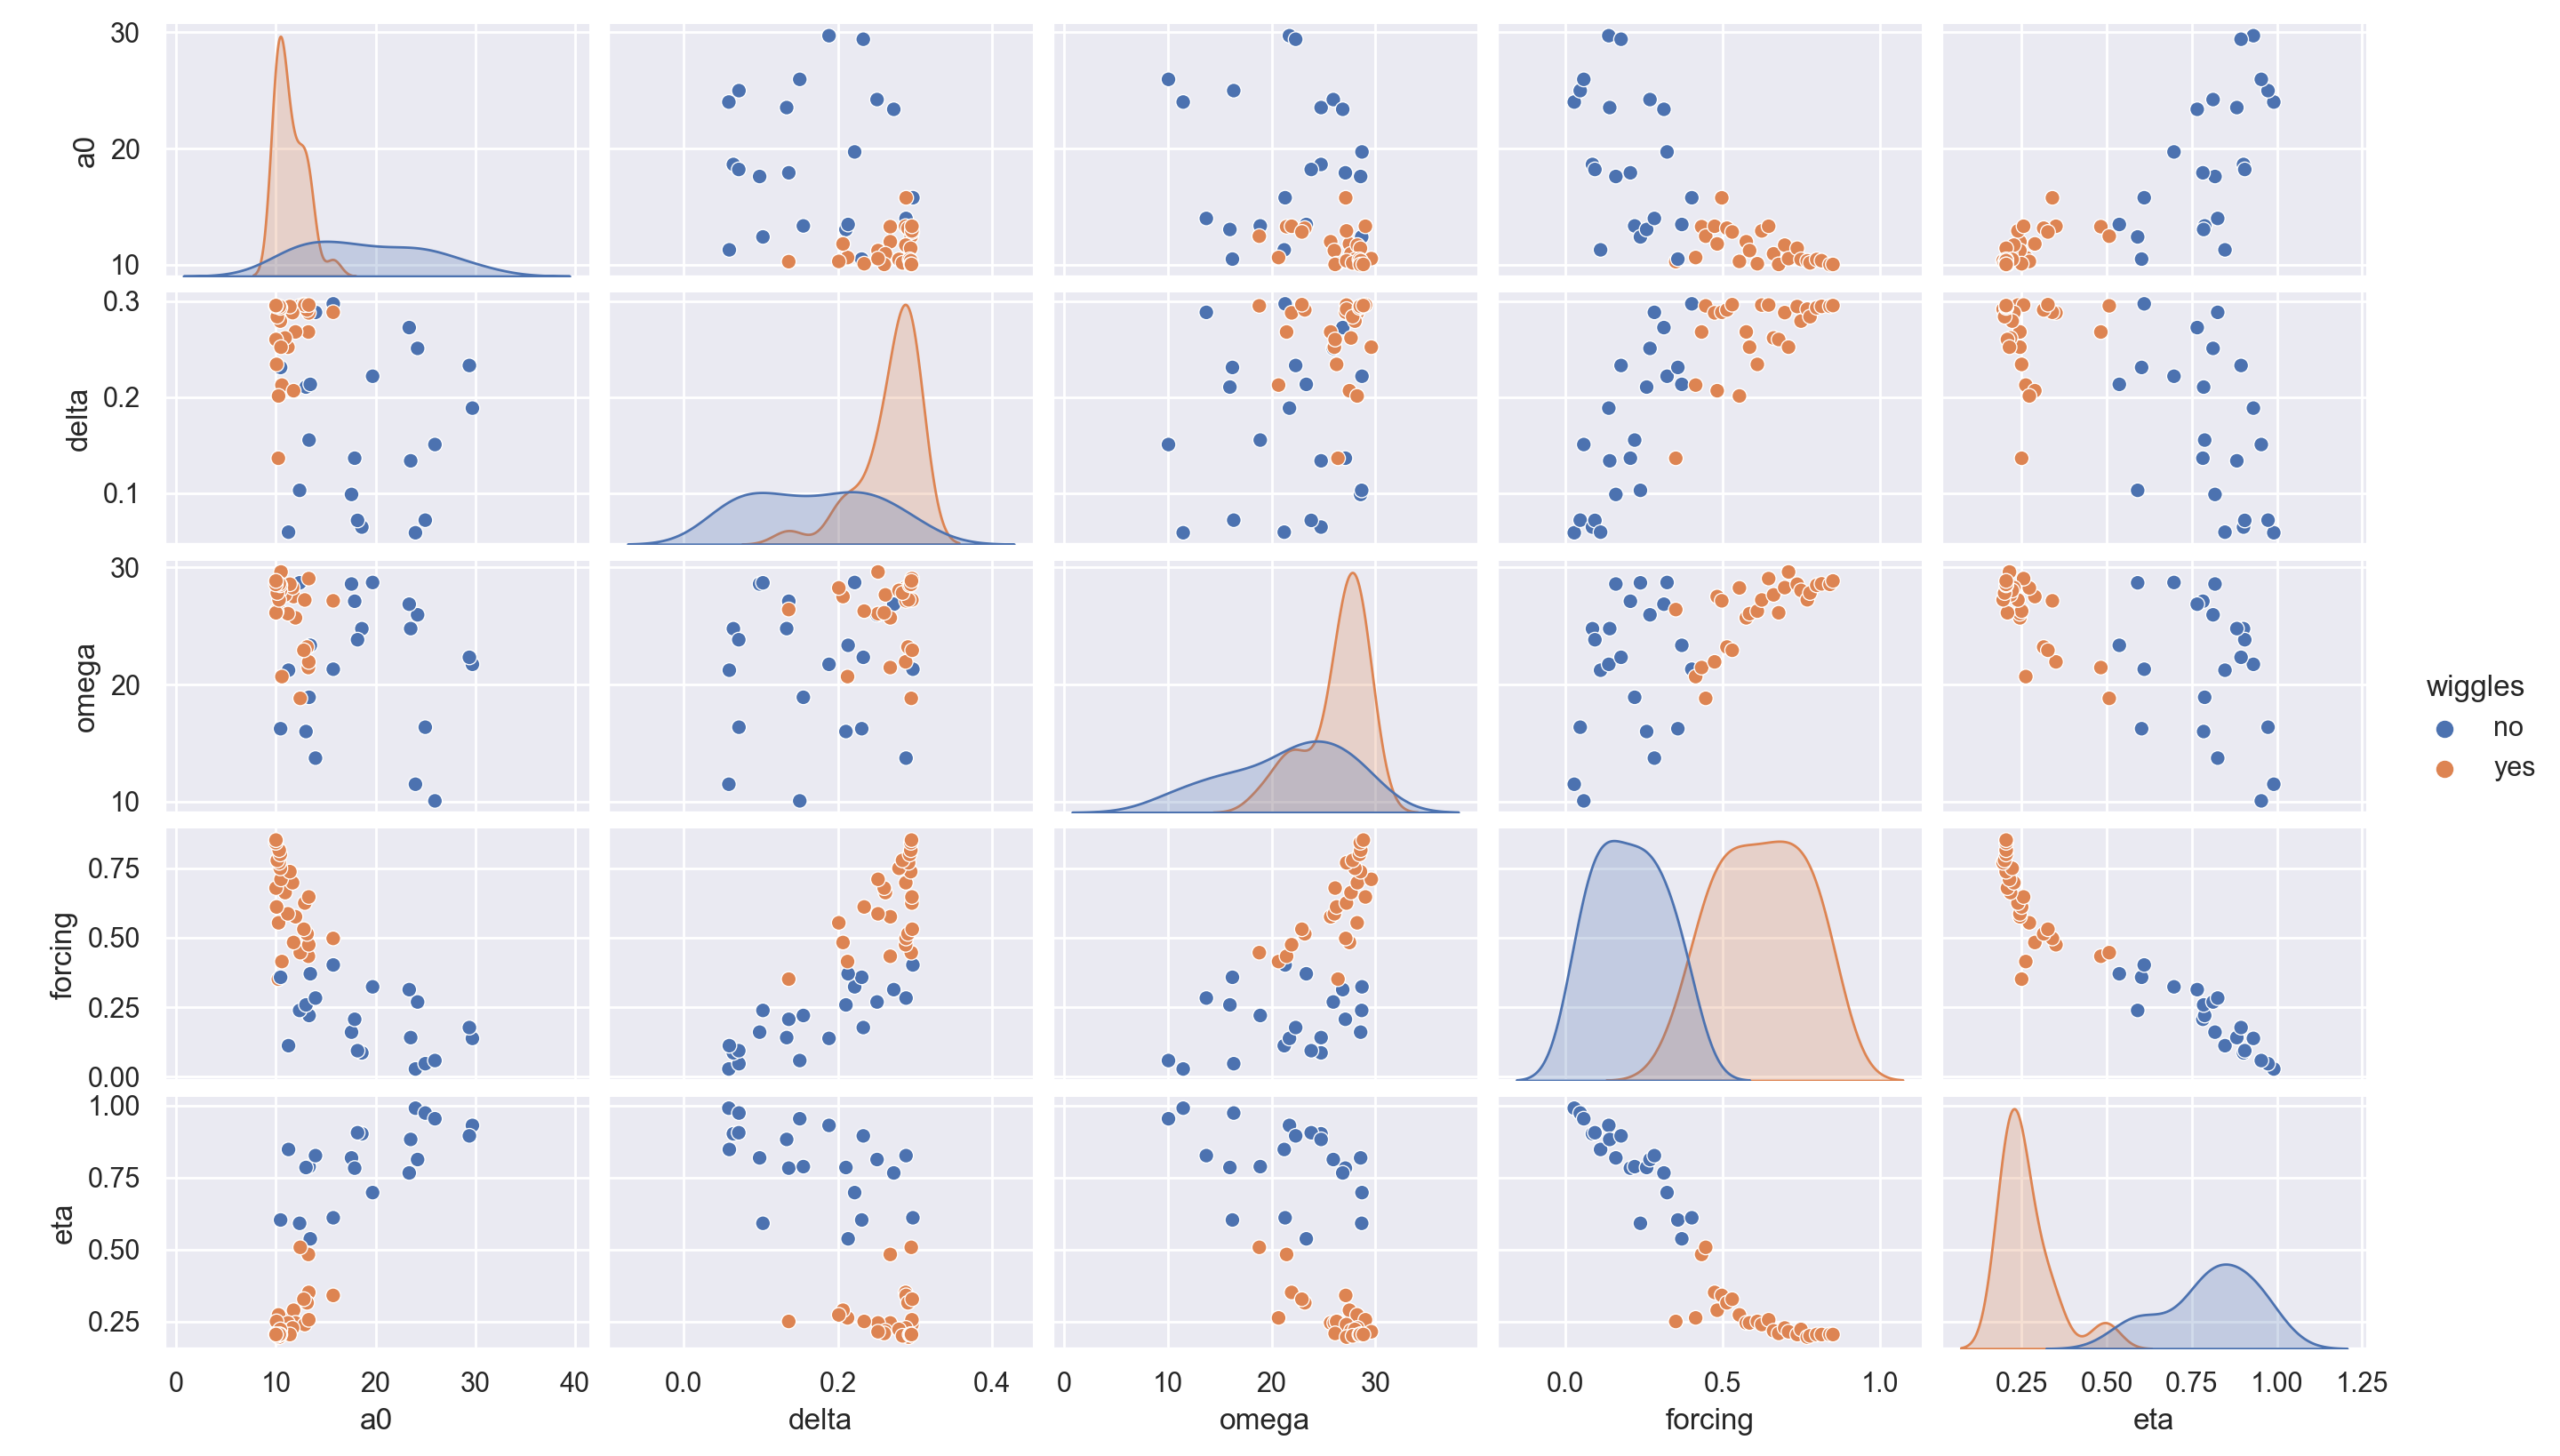
\includegraphics[width=1\columnwidth]{research_project/piston/figures/wiggles/wiggle_correlation.png}
%     \caption{Parameter space split by wiggle presence.
%     We observe how oscillations are prone to appear for low values in the speed of sound,
%     large values in displacement and frequency; that is, when the forcing into the system is larger than a given threshold $u_M$.}
%     \label{fig:wiggle_correlation}
% \end{figure}

\subsection{Non-Uniform Displacement}

\begin{table}[h]
    \centering
    \caption{Online operator approximation errors.}
    \begin{tabular}{lcccccc}
        \toprule
        {} &  Convection &    Mass &  N-Lifting &     RHS &  Stiffness &  Trilinear   \\
        p    &             &         &                    &         &            &            \\
        \midrule
        0.05 &     7.4e-01 & 3.6e-05 &            2.9e-02 & 4.2e-03 &    4.0e-08 &    2.5e-01 \\
        0.10 &     3.5e-02 & 2.1e-05 &            2.9e-02 & 4.6e-04 &    2.2e-08 &    6.8e-04 \\
        0.20 &     2.1e-02 & 1.7e-05 &            7.7e-03 & 9.7e-05 &    4.3e-09 &    5.1e-07 \\
        0.40 &     3.4e-03 & 3.2e-06 &            1.0e-03 & 1.4e-05 &    6.8e-10 &    1.5e-09 \\
        0.60 &     2.8e-04 & 2.4e-07 &            4.9e-05 & 1.5e-07 &    2.0e-11 &    4.1e-11 \\
        0.80 &     9.4e-06 & 4.8e-09 &            2.2e-06 & 3.2e-09 &    6.7e-13 &    3.3e-13 \\
        0.85 &     2.5e-06 & 2.6e-09 &            3.6e-07 & 2.5e-09 &    3.9e-13 &        -   \\
        0.90 &     6.6e-07 & 1.2e-09 &            1.9e-07 & 5.6e-10 &    4.2e-13 &        -   \\
        0.95 &     6.1e-07 & 6.3e-10 &            1.6e-07 & 2.7e-10 &    3.5e-13 &        -   \\
        1.00 &     1.7e-07 & 1.7e-10 &            6.5e-08 & 1.4e-10 &    4.8e-14 &    1.3e-15 \\
        \bottomrule
    \end{tabular}       
    \label{tab:arbitrary_displacement_errors_online}
\end{table}

\begin{table}[h]
    \centering
    \caption{Basis size according to percentile position.}
    \begin{tabular}{lcccccc}
        \toprule
        {} & Convection & Mass & N-Lifting & Rhs & Stiffness & Trilinear \\
        p    &            &      &                   &     &           &           \\
        \midrule
        0.05 &          1 &    1 &                 0 &   1 &         3 &         4 \\
        0.10 &          2 &    2 &                 1 &   3 &         6 &         9 \\
        0.20 &          4 &    4 &                 3 &   6 &        13 &        18 \\
        0.40 &          8 &    8 &                 7 &  12 &        27 &        37 \\
        0.60 &         12 &   12 &                11 &  19 &        40 &        56 \\
        0.80 &         16 &   16 &                15 &  25 &        54 &        75 \\
        0.85 &         17 &   17 &                16 &  27 &        57 &        79 \\
        0.90 &         18 &   18 &                17 &  28 &        61 &        84 \\
        0.95 &         19 &   19 &                18 &  30 &        64 &        89 \\
        1.00 &         20 &   21 &                19 &  32 &        68 &        94 \\
        \bottomrule
    \end{tabular}        
    \label{tab:arbitrary_displacement_size_percentile}
\end{table}

\begin{figure}[h]
    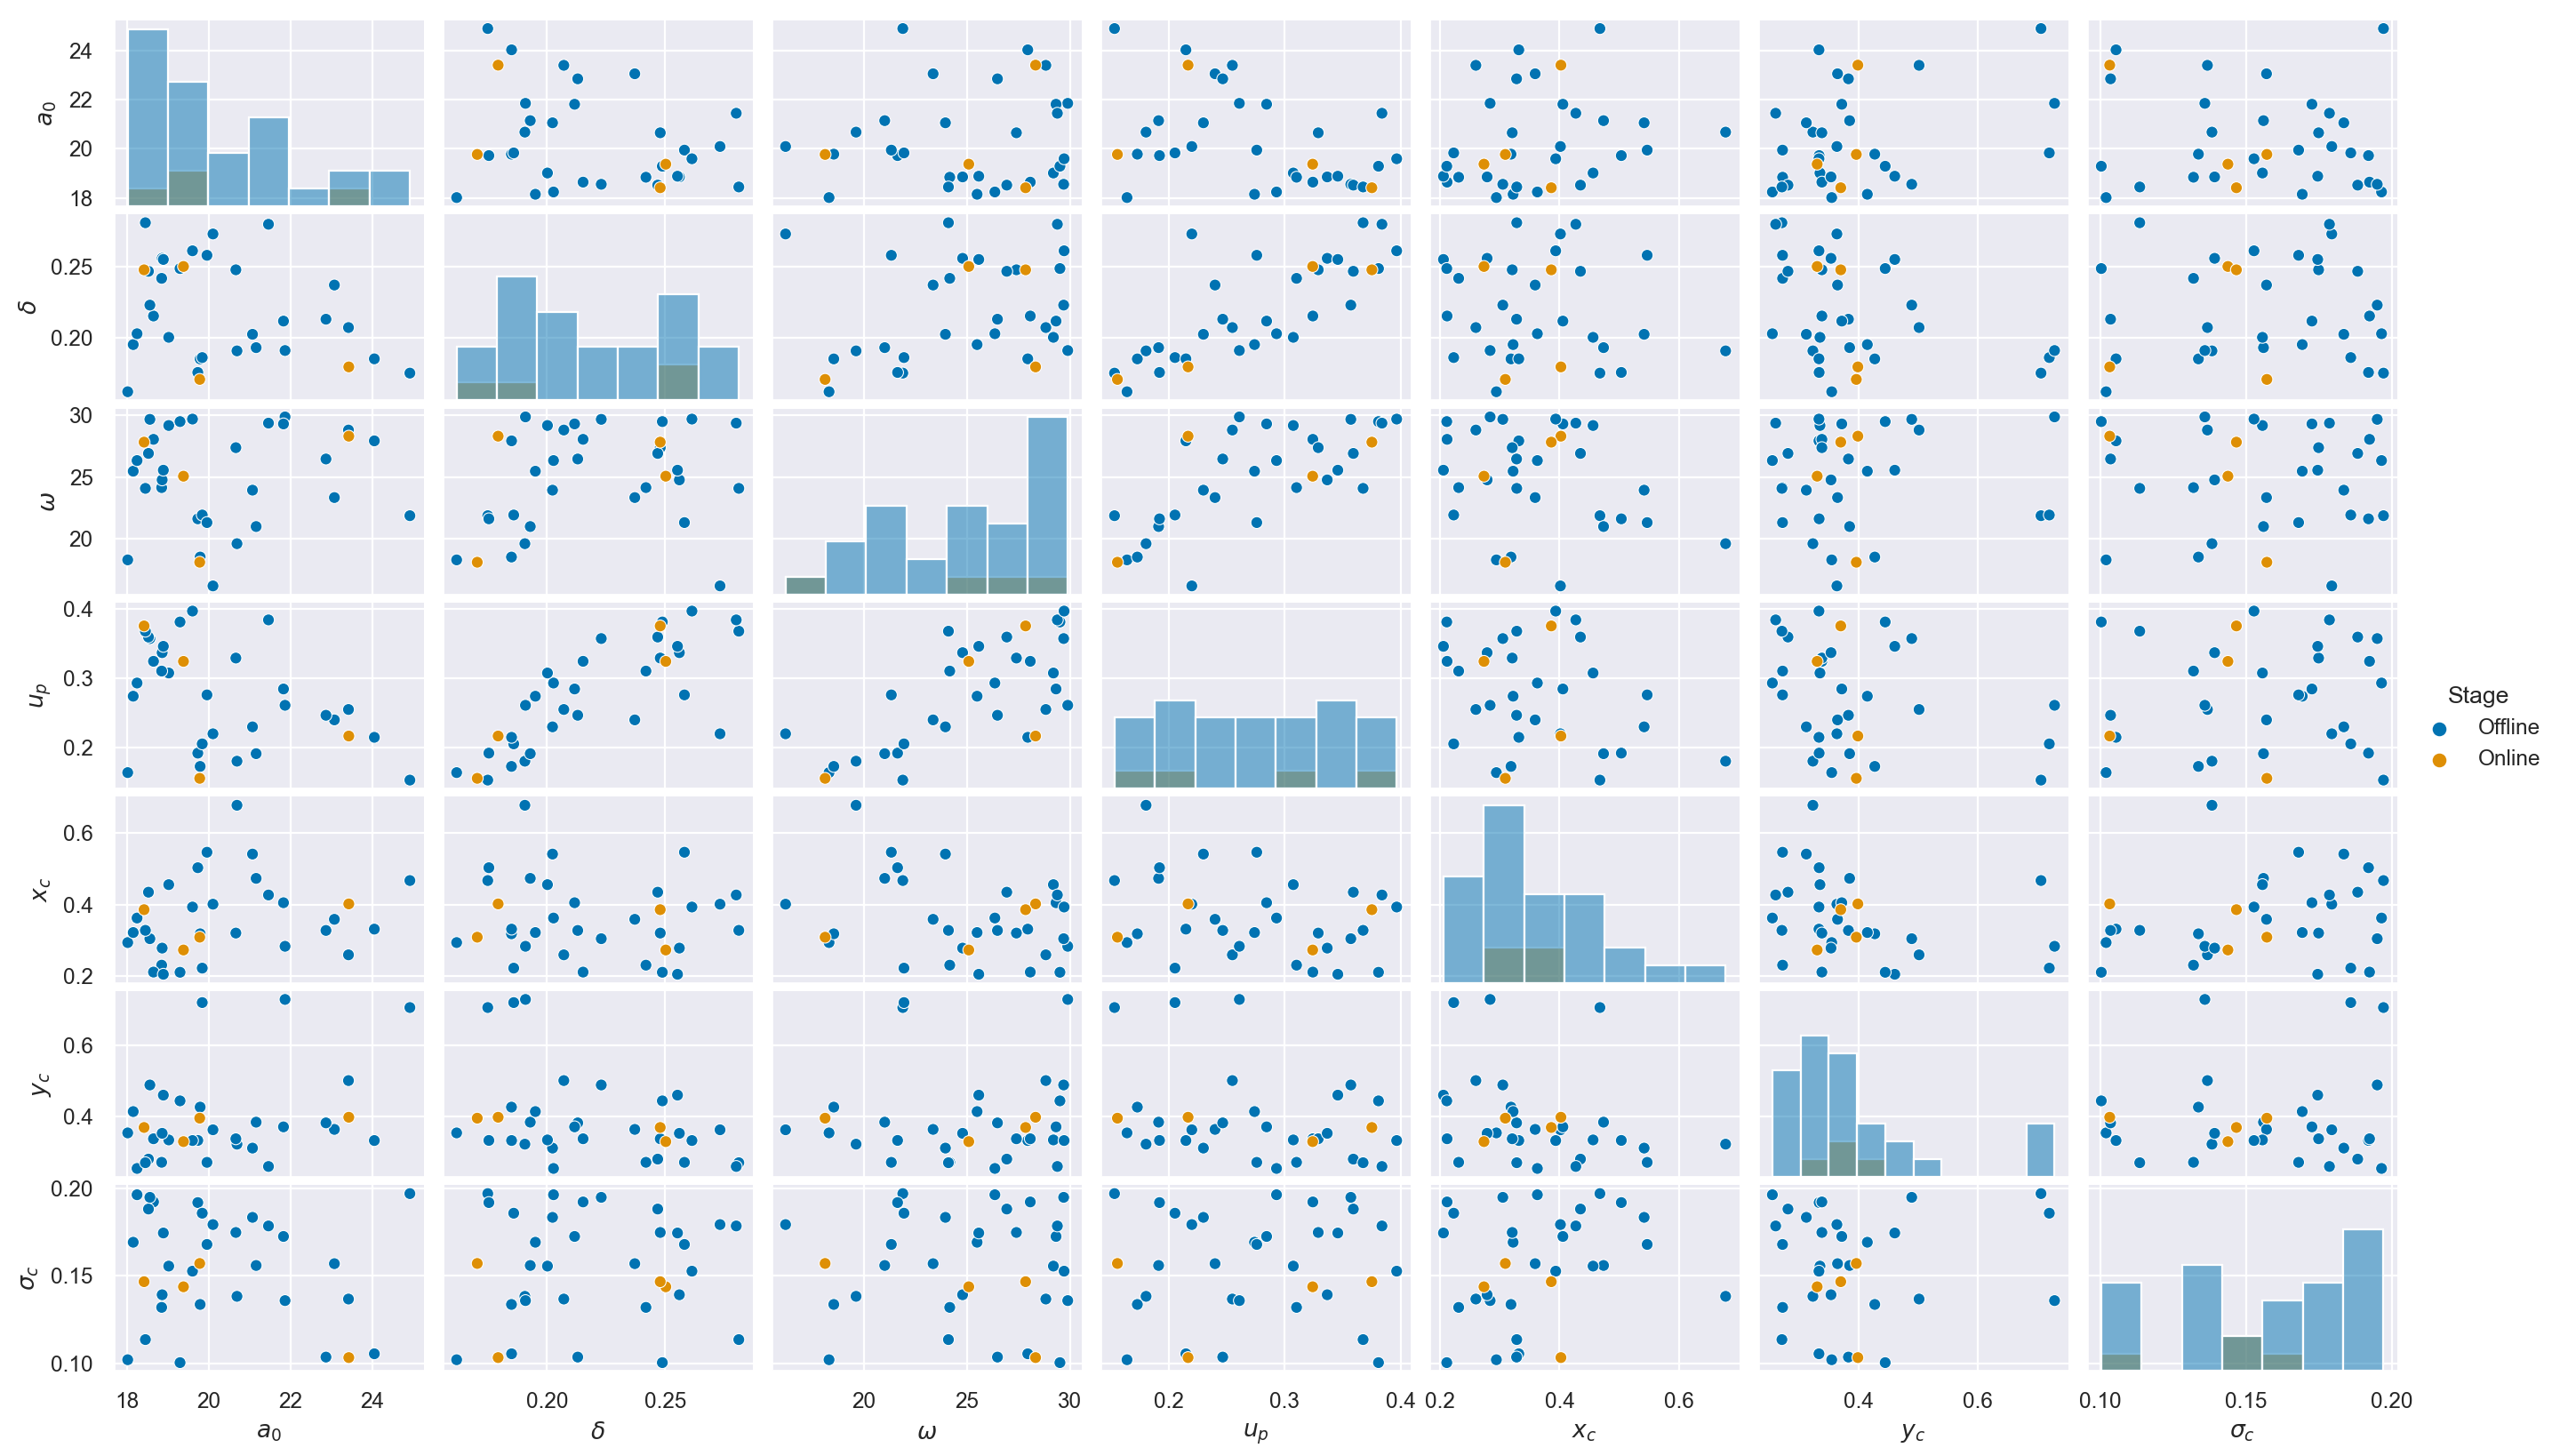
\includegraphics[width =\columnwidth]{research_project/piston/figures/nonlinear_displacement/separable/sampling_space.png}
    \caption{Sampling space for offline and online stages 
    for the nonlinear displacement test case.}
    \label{fig:nlinear_disp_operators_sampling_space}
\end{figure}

\end{document}